\documentclass{article}
\usepackage[]{color}

\usepackage{hyperref} % Almost certainly will need
\usepackage{fullpage} % Good for making PDFs as well
\usepackage{listings} % Needed to insert code
\usepackage{lstautogobble}
\usepackage{float}

\usepackage{graphicx}
\usepackage{textcomp}
\usepackage[T1]{fontenc}
% This makes it so the web pages don't have indents as most of the time
% they are just annoying
\setlength{\parindent}{0pt}
% Makes code in lstlisting copy-and-paste-able
\lstset{
  upquote=true,
  basicstyle = \ttfamily,
  columns=fullflexible
  escapeinside=||,
  autogobble
}
% --- This section allows for tex4ht only control statements
% From http://tex.stackexchange.com/questions/93852/what-is-the-correct-way-to-check-for-latex-pdflatex-and-html-in-the-same-latex
\makeatletter
\edef\texforht{TT\noexpand\fi
  \@ifpackageloaded{tex4ht}
    {\noexpand\iftrue}
    {\noexpand\iffalse}}
\makeatother

\newcommand{\code}[1]{\texttt{\textmd{#1}}}
\newcommand{\assertion}[2]{\textbf{Assertion: }#1 (\hyperlink{#2}{#2})}
\newcommand{\assertiondest}[1]{\hypertarget{#1}{#1:}}

\newif\ifComments
%\Commentstrue
\ifComments
\newcommand{\nelson}[1]{\noindent\textcolor{red}{Nelson: {#1}}}
\newcommand{\marcus}[1]{\noindent\textcolor{blue}{Marcus {#1}}}
\else
\newcommand{\nelson}[1]{}
\newcommand{\marcus}[1]{}
\fi


\begin{document}

% This is an example of using a switch to have pdf/html only code
\ifpdf
  \LARGE
  \textbf{Generator Assignment}
  \normalsize
\fi

For this assignment you will be building a parser for a number generator. The generator will
produce a series of numbers through an expression. Your task is to parse the generator statement,
interpret it, and print the numbers that should be produced by the generator. You will be using
\textit{Antlr4} to generate the \textbf{lexer} and \textbf{parser} for it. You will
then implement an interpreter in \textit{C++}. Documentation and tutorials for \textit{Antlr4} can
be found here \href{https://github.com/antlr/antlr4/blob/master/doc/index.md}
{Antlr4 documentation}

\section{Language Specification}
\subsection{Generator}
A generator generates a series of numbers based on an expression and bounds. In a sense it is
similar to a \textit{C} style \code{for} loop. For this assignment, the index variable will always
start at the lower bound and stop when it is greater than the upper bound. The generator will
always increment by the integer value 1. In \textit{C}, this would be:
\begin{lstlisting}
  for(int i = <start>; i <= <end>; ++i)
\end{lstlisting}

\subsubsection{Reserved Keywords}
The following keywords are reserved in \textit{Generator}.
\begin{itemize}
  \item \code{in}
\end{itemize}

\subsubsection{Generator Format}
The generator format will always follow the same format:
\begin{lstlisting}
  [ <id> in <int_1>..<int_2> | <expr>];
\end{lstlisting}

\begin{itemize}
  \item \code{id} is the identifier of a variable.
  \item{\code{int\_1}} is an integer representing the lower bound of the generator
  \item{\code{int\_2}} is an integer representing the upper bound of the generator
  \item{\code{expr}} is an expression
\end{itemize}

\assertion{\code{int\_1} and \code{int\_2} will never be expressions, only integer literals.}
{simple-bounds} \\
\assertion{\code{int\_1} will be never be greater than \code{int\_2}.}{sane-bounds}\\
\assertion{If an identifier is used in \code{expr} then it will match \code{id}.}{matching-id}

For this assignment the value of the identifier variable \code{<id>}:
\begin{enumerate}
  \item is initialized to the value of \code{int\_1}.
  \item is used to evaluate the expression.
  \item is incremented by one.
  \item stops when its value is greater than \code{int\_2}.
\end{enumerate}
For each value assumed by \code{id}, \code{expr} is used to generated the next number in the
series.

Examples of valid generators:
\begin{lstlisting}
  [i in 1..10 | i * i];
  [i in 0..10 | 2 ^ i];
\end{lstlisting}

In this assignment white space is not important so the following is valid:

\begin{lstlisting}
  [i
  in
  1
  ..
  10
  |
  i*i];
  [i in 1..10|2^i];
\end{lstlisting}

\assertion{Whitespace is guaranteed to be a space, a tab, a carriage return, or a new
line.}{simple-whitespace}

Because identifiers need white space to separate each other the following is invalid:
\begin{lstlisting}
  [iin1..10|i*i];
  [i in1..10|2^i];
\end{lstlisting}

\subsection{Identifier}
For the purpose of this assignment identifiers are simple. They must start with a character and
can be followed by any amount of numbers and characters. Identifiers cannot be key words.

Examples of valid identifiers:
\begin{lstlisting}
  hello
  h3llo
  Hi
  h3
\end{lstlisting}

Examples of invalid identifier:
\begin{lstlisting}
  in
  3d
  a-bad-variable-name
  no@twitter
  we.don't.like.punctuation
  not_at_all
\end{lstlisting}

\subsection{Integers}
In this assignment integer literals are defined as being a string that contains only the number
characters 0-9 with no spaces.

\assertion{All integer literals will be positive.}{positive-literals}\\
\assertion{All integer literals will fit in 31 unsigned bits.}{literal-size}

Examples of valid integers literals:
\begin{lstlisting}
  1
  123
  5234
  01
  10
\end{lstlisting}

Examples of invalid integers literals:
\begin{lstlisting}
  -1
  1.0
  one
  1_1
  1o
  4294967296
\end{lstlisting}

\subsection{Expression}
An expression is composed of integers, identifiers, and integer mathematical operations.

\subsubsection{Operators}
\begin{center}
  \begin{tabular}{|l|c|l|c|}
    \hline
    \textbf{Operation} & \textbf{Symbol} & \textbf{Usage} &
    \textbf{Associativity} \\
    \hline
    exponentiation & \textasciicircum & \code{expr \textasciicircum\ expr} & right\\
    multiplication & *  & \code{expr * expr}  & left \\
    division       & /  & \code{expr / expr}  & left \\
    modulus        & \% & \code{expr \% expr}  & left \\
    addition       & +  & \code{expr + expr}  & left \\
    subtraction    & -  & \code{expr - expr}  & left \\
    \hline
  \end{tabular}
\end{center}

\subsubsection{Valid Expressions}
Valid formats for expressions are
\begin{lstlisting}
  (<expr>)
  <expr> <op> <expr>
  <int>
  <id>
\end{lstlisting}

\begin{itemize}
  \item \code{expr} is an expression.
  \item \code{int} is an integer.
  \item \code{id} is the identifier of a variable.
\end{itemize}

\assertion{All expressions will result in a value that fits in a 32 bit signed integer.}
{expression-size}

Examples of valid expressions are
\begin{lstlisting}
  i * 2 * 10 + 4
  2 ^ 4 * 5
\end{lstlisting}

\subsubsection{Precedence}
Precedence determines what order operations are evaluated in. Precedence works as defined in the
following table:
\begin{center}
  \begin{tabular}{|c|c|}
    \hline
    \textbf{Precedence} & \textbf{Operations} \\
    \hline
    HIGHER & \textasciicircum \\
           & *,/,\% \\
    LOWER  & +,- \\
    \hline
  \end{tabular}
\end{center}

The higher the precedence the sooner the value should be evaluated. For example, in the expression
\begin{lstlisting}
1 + 2 * 3
\end{lstlisting}
\code{2 * 3} should be evaluated before \code{1 + 2}. This is because multiplication, division, and modulus
have higher precedence than addition and subtractions.

\subsubsection{Associativity}
When parsing expressions associativity determines in what order operators of the same precedence
should be evaluated in. For example:
\begin{lstlisting}
  1 / 2 * 3
\end{lstlisting}

In this example both division and multiplication have the same precedence; associativity determines
which operations are evaluated first. Left associative operations will form a parse tree like this:
\begin{figure}[H]
  \centering
  
\includegraphics{static/left-assoc-gen.png}
\end{figure}

An example of one of these operations is addition. Lets say we have the following expression:
\begin{lstlisting}
  1 + 2 + 3 + 4
\end{lstlisting}

Because addition is left associative it will form the following parse tree:
\begin{figure}[H]
  \centering
  
\includegraphics{static/left-assoc-plus.png}
\end{figure}

In parse trees, evaluation can only happen when a node's children are all leaves. Therefore
\code{1 + 2} will be evaluated first. The result of this will be pushed up and the following tree
will be created.
\begin{figure}[H]
  \centering
  
\includegraphics{static/left-assoc-plus-2.png}
\end{figure}

Next, \code{3 + 3} is evaluated, making
\begin{figure}[H]
  \centering
  
\includegraphics{static/left-assoc-plus-3.png}
\end{figure}

Most operations used in this assignment are left associative, but there are also operations that
are right associative and take this format:
\begin{figure}[H]
  \centering
  
\includegraphics{static/right-assoc-gen.png}
\end{figure}

An example of a right associative operation is the exponent symbol or \code{\textasciicircum}.
For example
\begin{lstlisting}
  2 ^ 3 ^ 4 ^ 5
\end{lstlisting}

should be evaluated like so:
\begin{math}
  2 ^ {\displaystyle 3 ^ {\displaystyle 4 ^ {\displaystyle 5 }}}
\end{math}

In order for this expression to be evaluated correctly the following parse tree must be generated
\begin{figure}[H]
  \centering
  
\includegraphics{static/right-assoc-pow.png}
\end{figure}

For a more complex example let's take the expression:
\begin{lstlisting}
1 + 2 * 3 + 1 / 3 ^ 4 ^ (6 * 3)
\end{lstlisting}

This should generate the following parse tree:
\begin{figure}[H]
  \centering
  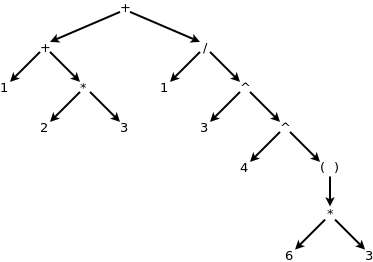
\includegraphics{static/assoc-example.png}
\end{figure}

\section{Output}
Output is standardized to ensure everyone can pass everyone's tests. All the numbers generated by
the generator will be printed on the same line with spaces separating each number. There
\textit{should} be a new line after each generator's output. There \textit{should not} be a
trailing space after the final number and before the newline. There \textit{should} be an empty
line at the end of your output.

Example input:
\begin{lstlisting}
  [i in 1..10| i];
  [x in 0..3| x-1];
  [x in 1..4| 10];
\end{lstlisting}

Expected Output:
\begin{lstlisting}
1 2 3 4 5 6 7 8 9 10
-1 0 1 2
10 10 10 10
\end{lstlisting}

This may be rendered incorrectly on your platform, therefore, this\
\href{https://webdocs.cs.ualberta.ca/\%7Ec415/generator/static/ex.in} {test case} and its
\href{https://webdocs.cs.ualberta.ca/\%7Ec415/generator/static/ex.out} {output} are available to
test for yourself. Do not include this test in your submission.

\section{Assertions}
\textbf{ALL} input will be valid. It can be a good idea to do error checking for your own
testing and debugging, but it is \textit{not necessary}. What does it mean to be valid input?
See these rules:
\begin{enumerate}
  \item
    \assertiondest{undef-behaviour}
    A test case \textit{will not} take advantage of undefined behaviour. Undefined behaviour is
    functionality that does not have an outcome described explicitly by this specification.
  \item
    \assertiondest{simple-bounds}
    The bounds on the index variable will always be integer literals and never an expression. For
    example, the following test would be considered invalid:
    \begin{lstlisting}
      [i in (1-1)..1 | i];
    \end{lstlisting}
  \item
    \assertiondest{sane-bounds}
    The bounds on the index variable will always be such that $\code{int\_1} \leq
    \code{int\_2}$. For example, the following test would be considered invalid:
    \begin{lstlisting}
      [i in 1..0 | i];
    \end{lstlisting}
  \item
    \assertiondest{matching-id}
    Any variable used in an expression will match the variable defined in the generator. For
    example, the following test would be considered invalid:
    \begin{lstlisting}
      [i in 0..1 | j];
    \end{lstlisting}
  \item
    \assertiondest{simple-whitespace}
    Whitespace is guaranteed to be a space, a tab, a carriage return, or a new
    line. Any other whitespace characters will render the input invalid. The following ANTLR rule
    will ensure you adhere to this:
    \begin{lstlisting}
      WS : [ \t\r\n]+ -> skip;
    \end{lstlisting}
  \item
    \assertiondest{positive-literals}
    All integer literals will be positive. For example, the following tests would be considered
    invalid:
    \begin{lstlisting}
      [i in 0..1 | -1];
      [i in -2..-1 | i];
    \end{lstlisting}
  \item
    \assertiondest{literal-size}
    All integer literals will fit in 31 unsigned bits. This means an integer literal can be
    anywhere in the range $[0, 2^{31} - 1]$ or $[0, 2147483647]$. For example, the following tests
    would be considered invalid:
    \begin{lstlisting}
      [i in 0..1 | -1];
      [i in 0..1 | 2147483648];
      [i in 0..2147483648 | 0];
      [i in -1..1 | 0];
    \end{lstlisting}
  \item
    \assertiondest{expression-size}
    All expressions will result in a value that fits in a 32 bit signed integer. This means the
    result of an expression can be anywhere in the range $[-2^{31}, 2^{31} - 1]$ or $[-2147483648,
    2147483647]$. Any operation that results in underflow or overflow will render the input
    invalid. For example, the following tests would be considered invalid:
    \begin{lstlisting}
      [i in 0..1 | 2147483647 + 1];
      [i in 0..1 | 0 - 2147483647 - 2];
    \end{lstlisting}
\end{enumerate}
If you encounter what you think is undefined behaviour or think something is ambiguous then
\textit{do} make a forum post about it. While the generator is a relatively small spec,
the latter assignments \textit{will not be}.

\section{Provided Frameworks}

The following tools have been provided for you to make development and testing easier

\subsection{Project Layout}
For the tools provided to work your project should be in the specified layout.

\begin{lstlisting}
+-- cmake
|   +-- antlr_generate.cmake
|   +-- get_antlr.cmake
|   +-- get_antlr_manual.cmake
|   +-- symlink_to_bin.cmake
+-- CMakeLists.txt
+-- grammar
|   +-- Generator.g4
+-- include
|   +-- placeholder.h
+-- README.md
+-- src
    +-- CMakeLists.txt
    +-- main.cpp
+-- tests
    +-- Input
        +-- ...
    +-- Output
        +-- ...
\end{lstlisting}


\subsection{Makefile}
The \texttt{Makefile} provided is an exact copy of the one that will be used for grading.  Any changes made to
this makefile will not exist in the one used for grading so as a rule of thumb don't change it. The project must
be in the specified layout for the makefile to properly work (see \texttt{Project Layout})

The makefile has the following commands:
\begin{itemize}
  \item{\textbf{all}}: Builds all solution files
  \item{\textbf{run}}: Runs the solution (builds solution if necessary) takes f="<filename>" as an argument for
    input file
  \item{\textbf{test}}: Runs testing system against solution (builds solution if necessary)
  \item{\textbf{clean}}: Cleans all generated files including IntelliJ generated files
  \item{\textbf{submissible}}: Collects files for submission and places them in a tar ball. This file contains
  the files in the format they should be in
\end{itemize}

\subsection{generator\_tester}
This program runs all your test files against their matching outputs. This program is designed to operate in the
same manor as how the marking script will test solutions. For best results have \textit{colordiff} installed.

Help for generator tester can be found by running with the -h flag:
\begin{lstlisting}
  ./generator_tester -h
\end{lstlisting}

It by default expects that all input Tests are in \texttt{TestFiles/Input/} and that  all output files are in
\texttt{TestFiles/Output/}

\section{Deliverables}
To prepare your project for delivery use the Makefile provided and use the \texttt{submissible} command. Ex:
\begin{lstlisting}
  make submissible
\end{lstlisting}

The makefile will prompt you to enter your CCID (not your student id number). This should create a file called:
\begin{lstlisting}
  submission_<CCID>.tar.gz
\end{lstlisting}

This submission file will contain your \texttt{src} folder, \texttt{TestFiles}, and your README
\begin{lstlisting}
  +-- submission_<CCID>.tar.gz
    +-- README
    +-- src/
      +--  Main.Java
      +-- *.g4
      +-- *.Java
    +-- TestFiles/
      +-- Input/
        +-- (testfiles)
        +-- test_01
        +-- test_02
        +-- ...
      +-- Output/
        +-- (matching output files. Names must match between input test and output test)
        +-- test_01
        +-- test_02
        +-- ...
\end{lstlisting}

\section{Tips and Hints}
\begin{enumerate}
  \item Write tests \textbf{BEFORE} you implement the things they will test. The testing script provide is
  designed to handle failed test cases. You can turn off stopping on invalid output and you can also turn off
  displaying erroneous output with the flags "-a and -s" respectively.
  \item First and foremost \textbf{READ THE DOCUMENTATION FOR ANTLR4} here is the link again
    \href
    {https://github.com/antlr/antlr4/blob/master/doc/index.md}
    {Antlr4 documentation}.
  \item \textit{Antlr4} has two ways of navigating the parse tree, Visitors and Listeners. For this assignment use the
    visitor method. For the next assignment you'll use either but for this assignment the visitor is better
    suited.
  \item Remember that in the lexer the order of when tokens are defined is very important. The lexer will try to
    follow the first rule it can.
  \item \textit{Antlr4} has no standardized naming convention or style guide. This means you \textbf{CAN} do whatever you
    want for style. With that in mind I highly recommend you follow something similar to the one on the \textit{Antlr4}
    documentation pages. What ever you choose make sure it is easy to read and is consistent as \textbf{part of
    your grade} will be based of your software design and that includes code legibility.
\end{enumerate}

\end{document}
